% Relatório parcial (1ª entrega) -- CIN0020 Sinais e Sistemas 2026.2
% Compilar no Overleaf com pdfLaTeX. Figuras em figuras/ (geradas por figuras_relatorio.py).
\documentclass[10pt,a4paper]{article}

\usepackage[utf8]{inputenc}
\usepackage[T1]{fontenc}
\usepackage{lmodern}
\usepackage[brazil]{babel}
\usepackage[a4paper,margin=1.8cm]{geometry}
\usepackage{amsmath}
\usepackage{graphicx}
\usepackage{booktabs}
\usepackage[font=small,labelfont=bf,skip=3pt]{caption}
\usepackage{float}
\usepackage{enumitem}
\usepackage[hidelinks]{hyperref}

\setlist{nosep,leftmargin=*}
\setlength{\parskip}{2pt}
\setlength{\textfloatsep}{6pt}
\setlength{\floatsep}{5pt}
\setlength{\intextsep}{5pt}

\newcommand{\cod}[1]{\texttt{#1}}

\begin{document}

% ------------------------------------------------------------------ capa
\begin{titlepage}
  \centering
  \vspace*{3cm}
  {\large CIN0020 -- Sinais e Sistemas -- 2026.2\par}
  \vspace{1.5cm}
  {\LARGE\bfseries Análise de sinais de vibração de drones e\\ classificação de condições das hélices\par}
  \vspace{0.8cm}
  {\Large Relatório parcial -- 1ª entrega\par}
  \vspace{2cm}
  {\large
  Silvanio da Silva Assunção\\
  % TODO: preencher os nomes dos demais integrantes
  [Nome 2]\\
  [Nome 3]\par}
  \vfill
  {Código e notebooks: \url{https://github.com/silvanio45/drone-vibration-analysis}\par}
  \vspace{0.5cm}
  {Recife, novembro de 2026\par}
\end{titlepage}

% ------------------------------------------------------------------ 1
\section{Contextualização e objetivo}

Danos em hélices podem alterar a intensidade e o conteúdo em frequência das vibrações de um drone.
O objetivo é analisar sinais reais de aceleração de drones com hélices saudáveis e defeituosas, extrair e interpretar características nos domínios do tempo e da frequência e comparar o que cada domínio revela.
Esta entrega cobre a preparação dos dados, as duas análises, a comparação entre domínios e uma investigação adicional.
O código está nos notebooks 1 a 6 do repositório indicado na capa.

% ------------------------------------------------------------------ 2
\section{Dataset, registros escolhidos e preparação}

\textbf{Dataset e sensor.} O DronePropB~\cite{dronepropb} tem 111 arquivos \cod{.mat}, nomeados \cod{F\#\_SV\#\_SP\#\_C\#[\_R\#]}.
Cada arquivo tem o \cod{AccData} (1 canal, $f_s = 10$\,kHz, conferida pelo vetor de tempo nos 111 arquivos) e, em 108 deles, a \cod{IMUData} (3 canais, 1\,kHz).
Usamos só o \cod{AccData}.
A IMU tem de 2 a 4\,s de partida e parada, offset de $\approx 9{,}7$ no canal 3 (compatível com a gravidade) e Nyquist de 500\,Hz.
O \cod{AccData} é estável do início ao fim e tem média de $\approx -0{,}001$.
A documentação não define a unidade do \cod{AccData}, que tratamos como unidade arbitrária (u.a.), nem os códigos do nome.
Pelo dataset irmão DronePropA~\cite{dronepropa}, \cod{F0} é saudável, \cod{F1}--\cod{F3} são tipos de falha e \cod{SV} é a severidade.
O \cod{SP} foi inferido dos dados como nível de velocidade, porque o pico principal sobe com ele (Seção~\ref{sec:investigacao}).
O significado de \cod{C} é desconhecido.

\textbf{Seleção, verificação e tratamentos.} Removemos 9 saudáveis \cod{C2} com sinal idêntico, pelo hash, ao \cod{C1} de mesmo \cod{SP} e \cod{R}, e os 3 de \cod{SP0}, que só existem para saudáveis.
Restam 99 registros: 18 saudáveis e 81 defeituosos.
Não há NaN, os extremos ocorrem em 1 ou 2 amostras por registro (sem saturação), e a razão entre o maior e o menor desvio por janela é no máximo 1,95.
Por isso, nenhum recorte foi aplicado.

\textbf{Justificativa da comparação.} Saudável e defeituosa são comparadas no mesmo \cod{SP} e \cod{C}, com o mesmo sensor, a mesma taxa e o mesmo janelamento (Tabela~\ref{tab:registros}).
O \cod{SP} muda a amplitude em uma ordem de grandeza e desloca os picos, e o \cod{C} muda o RMS dos saudáveis em até 4,4 vezes.
Os defeituosos \cod{C2} são comparados com os saudáveis \cod{C1} do mesmo \cod{SP}.

\begin{table}[H]
  \centering\small
  \caption{Registros usados em cada nível de \cod{SP} (iguais nos três níveis; duração do \cod{AccData} entre parênteses).}
  \label{tab:registros}
  \begin{tabular}{lccc}
    \toprule
    \cod{C} & Saudáveis (\cod{F0}, \cod{R1}--\cod{R3}) & Defeituosos (\cod{F1}--\cod{F3} $\times$ \cod{SV1}--\cod{SV3}) & Comparação \\
    \midrule
    \cod{C1} & 3 (60\,s) & 9 (60\,s) & no mesmo \cod{SP} e \cod{C} \\
    \cod{C2} & -- (cópias de \cod{C1}) & 9 (60\,s) & com os saudáveis \cod{C1} \\
    \cod{C3} & 3 (20 ou 60\,s) & 9 (20\,s) & no mesmo \cod{SP} e \cod{C} \\
    \midrule
    Total & 6 & 27 & \\
    \bottomrule
  \end{tabular}
\end{table}

\textbf{Janelamento.} Janelas de 2\,s ($N = 20000$, sem sobreposição), com $\Delta f = f_s/N = 0{,}5$\,Hz.
São 2370 janelas (480 saudáveis e 1890 defeituosas), cada uma ligada ao seu registro de origem.
Como as janelas de um registro não são independentes, as comparações também usam a mediana de cada registro.

\textbf{Limitação.} Pelo campo \cod{AccData.DATE}, os 81 defeituosos foram gravados em setembro de 2024, mas 12 dos 18 saudáveis (\cod{R2} e \cod{R3}) são de novembro.
Diferenças entre condições podem conter um efeito da sessão de gravação, o que verificamos nas Seções~\ref{sec:comparacao} e~\ref{sec:investigacao}.

% ------------------------------------------------------------------ 3
\section{Domínio do tempo}
\label{sec:tempo}

Para cada janela $x[n]$ calculamos:
\begin{itemize}
  \item média $\mu = \frac1N\sum x[n]$;
  \item potência média $P = \frac1N\sum x[n]^2$ (u.a.$^2$);
  \item $\mathrm{RMS} = \sqrt P$;
  \item desvio padrão $\sigma = \sqrt{\frac1N\sum (x[n]-\mu)^2}$, com divisor $N$, o que garante $P = \mu^2 + \sigma^2$;
  \item pico absoluto $\max|x[n]|$;
  \item pico a pico $\max x - \min x$;
  \item fator de crista $= \text{pico absoluto}/\mathrm{RMS}$, adimensional (vale $\sqrt2$ para uma senoide).
\end{itemize}
As demais medidas estão em u.a.
A Figura~\ref{fig:pares} (em cima) mostra sinais saudável e defeituoso com o mesmo \cod{SP} e \cod{C}, no mesmo trecho.
A Figura~\ref{fig:box_tempo} e a Tabela~\ref{tab:tempo} resumem as características.

\begin{figure}[H]
  \centering
  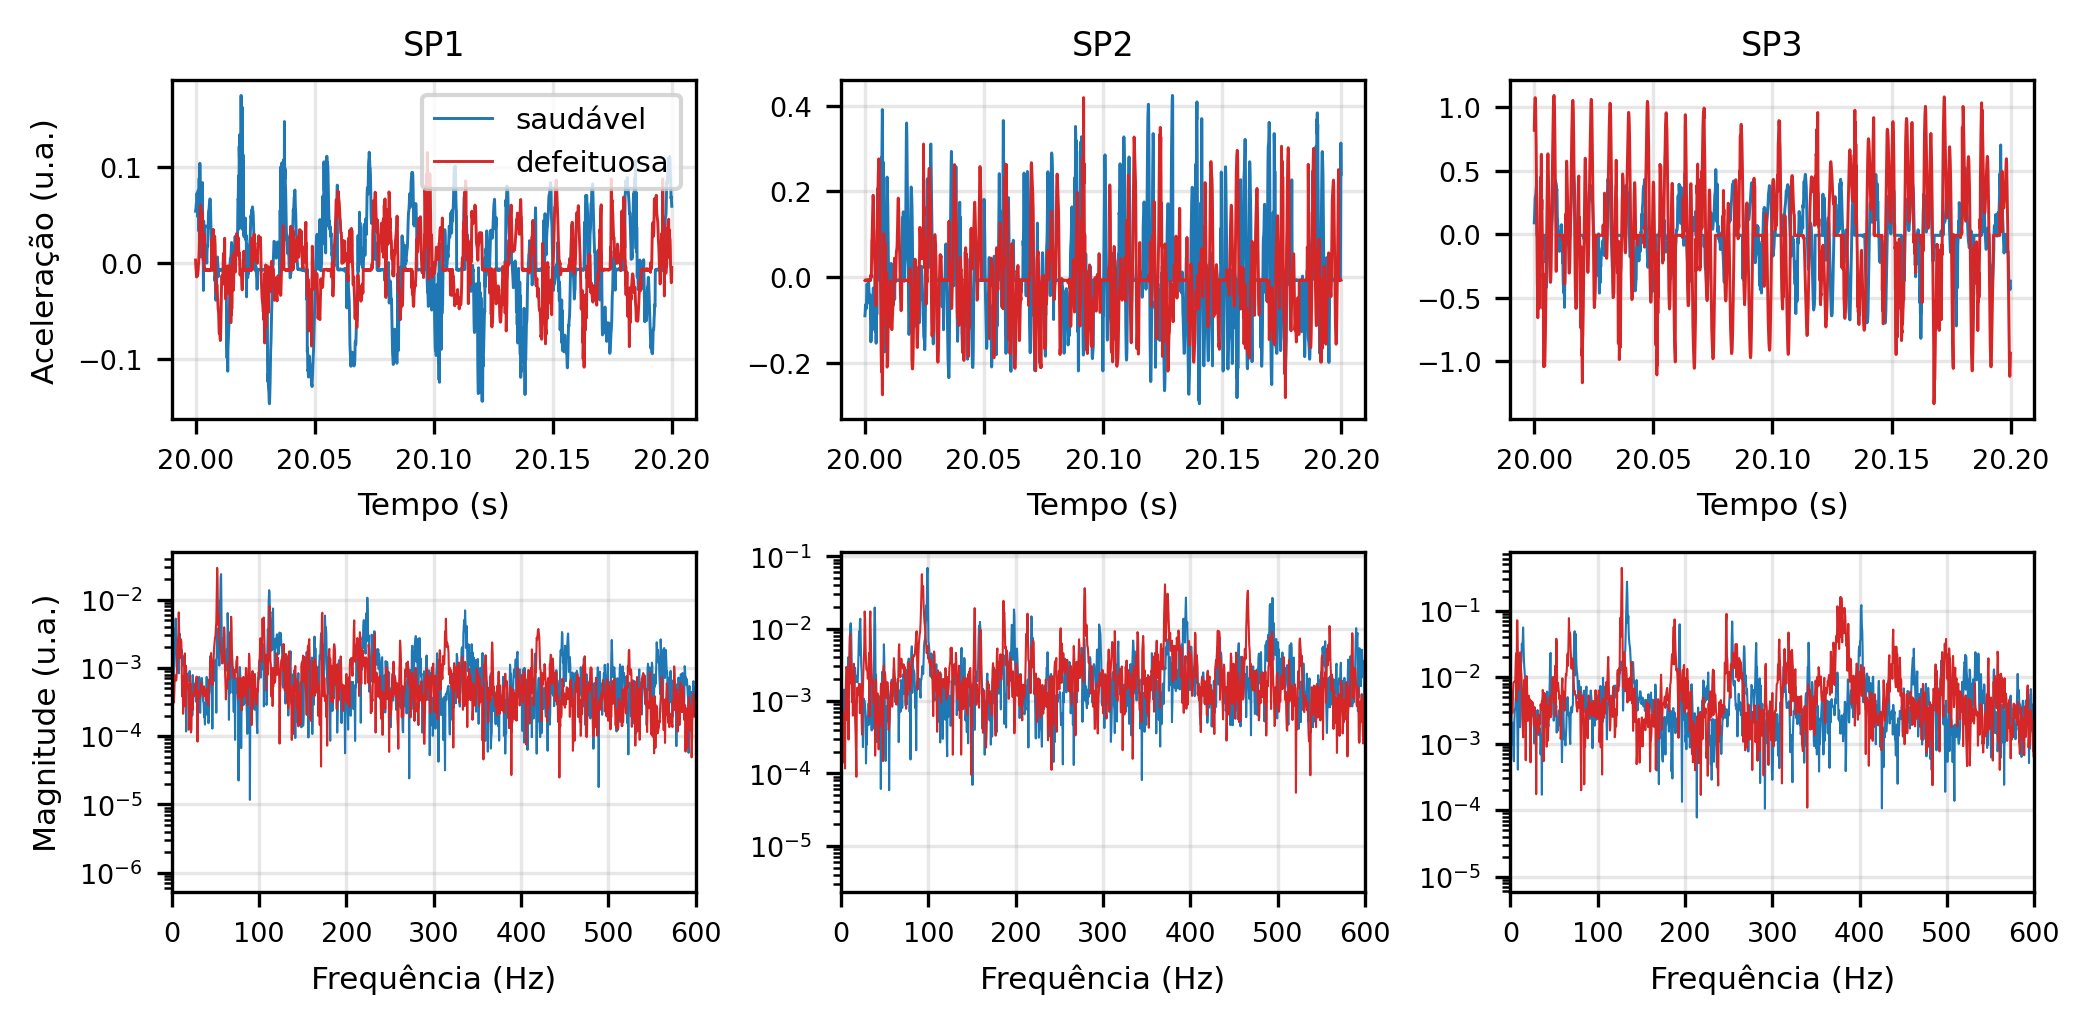
\includegraphics[width=\linewidth]{figuras/rel_pares.png}
  \caption{Saudável (\cod{F0\_SV0\_SP$k$\_C1\_R1}) $\times$ defeituosa (\cod{F1\_SV3\_SP$k$\_C1}). Em cima: \cod{AccData} de 20,0 a 20,2\,s. Embaixo: espectro de magnitude da janela de 20 a 22\,s.}
  \label{fig:pares}
\end{figure}

\begin{figure}[H]
  \centering
  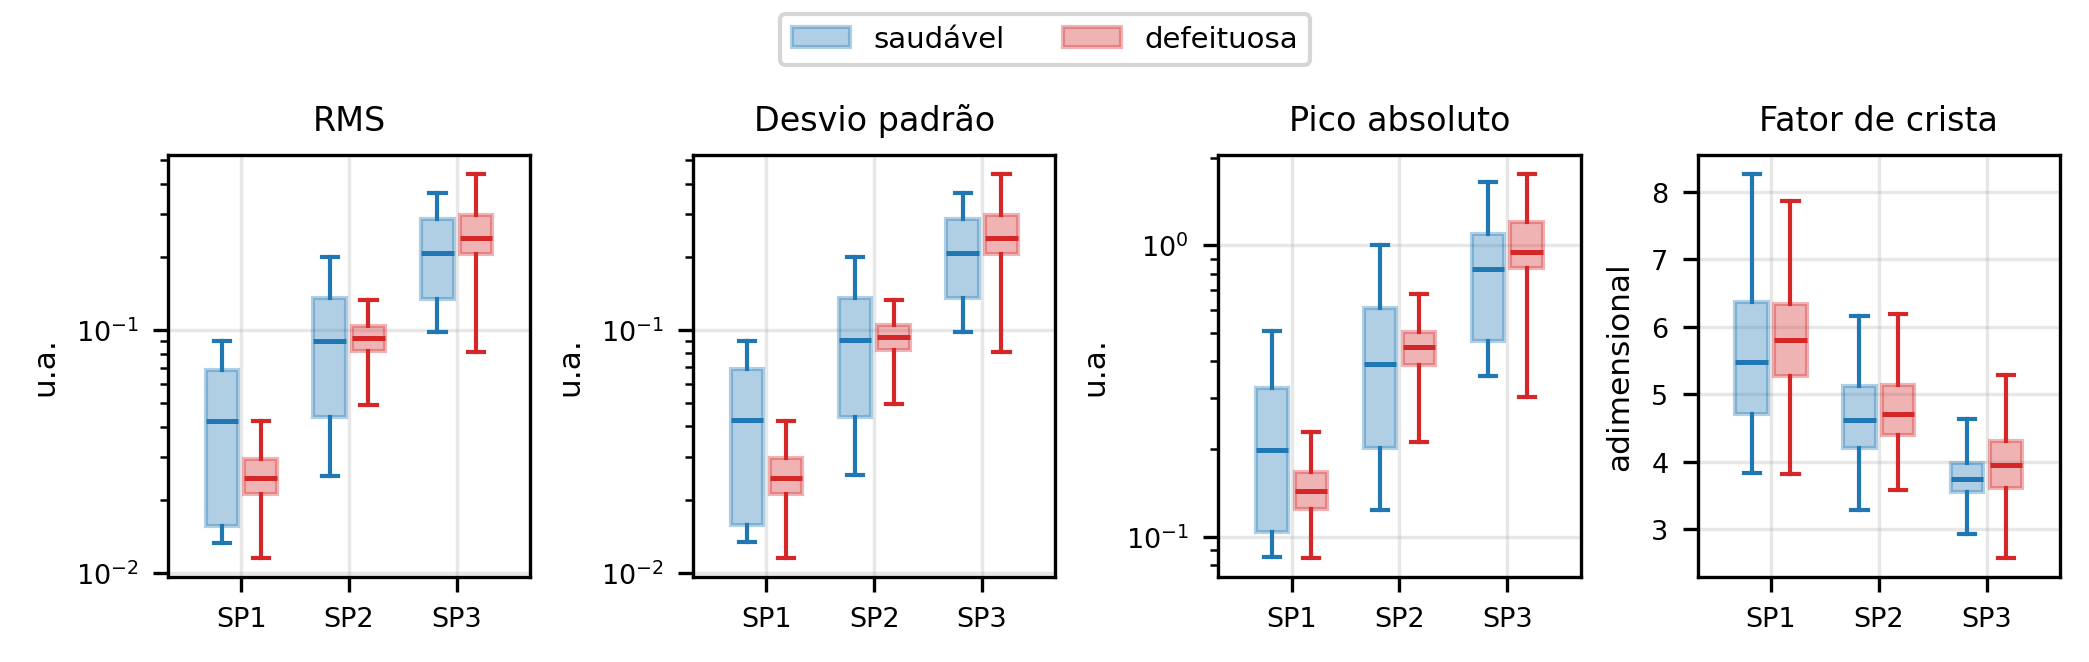
\includegraphics[width=\linewidth]{figuras/rel_box_tempo.png}
  \caption{Características temporais por janela de 2\,s, separadas por \cod{SP} (sem outliers).}
  \label{fig:box_tempo}
\end{figure}

\begin{table}[H]
  \centering\small
  \caption{Mediana das janelas por \cod{SP} e condição (S = saudável, D = defeituosa; IQR do RMS entre parênteses).}
  \label{tab:tempo}
  \begin{tabular}{lcccccc}
    \toprule
    & \multicolumn{2}{c}{\cod{SP1}} & \multicolumn{2}{c}{\cod{SP2}} & \multicolumn{2}{c}{\cod{SP3}} \\
    \cmidrule(lr){2-3}\cmidrule(lr){4-5}\cmidrule(lr){6-7}
    & S & D & S & D & S & D \\
    \midrule
    Média ($10^{-3}$ u.a.) & $-0{,}81$ & $-1{,}09$ & $-0{,}84$ & $-1{,}13$ & $-0{,}99$ & $-1{,}47$ \\
    RMS (u.a.) & 0,042 (0,053) & 0,025 (0,009) & 0,090 (0,091) & 0,093 (0,022) & 0,207 (0,15) & 0,239 (0,093) \\
    Pico absoluto (u.a.) & 0,198 & 0,143 & 0,393 & 0,448 & 0,829 & 0,952 \\
    Pico a pico (u.a.) & 0,382 & 0,249 & 0,757 & 0,837 & 1,561 & 1,807 \\
    Fator de crista & 5,48 & 5,80 & 4,61 & 4,70 & 3,75 & 3,95 \\
    \bottomrule
  \end{tabular}
\end{table}

\textbf{Interpretação.}
\begin{itemize}
  \item \textbf{O defeito não está associado a uma vibração sempre mais intensa.} O RMS da defeituosa é 0,58 vez o da saudável em \cod{SP1}, 1,03 em \cod{SP2} e 1,15 em \cod{SP3}. Os picos seguem o mesmo padrão.
  \item \textbf{Os saudáveis variam mais}, com IQR maior, por efeito do \cod{C} e da data. Por exemplo, os de novembro têm RMS de 0,074 contra 0,044\,u.a. do de setembro em \cod{SP1}/\cod{C1}. Comparando só registros de setembro, o RMS fica próximo na maioria dos grupos.
  \item \textbf{O fator de crista é ligeiramente maior na defeituosa nos três \cod{SP}}, mas a diferença é pequena perto da dispersão.
  \item \textbf{RMS e potência média trazem a mesma informação} ($\mathrm{RMS} = \sqrt P$). A potência só amplia as diferenças, por depender do quadrado da amplitude.
  \item \textbf{A componente média é desprezível.} $\mu^2/P$ tem mediana de 0,19\%, 0,017\% e 0,004\% em \cod{SP1}--\cod{SP3}, logo $\mathrm{RMS} \approx \sigma$.
  \item \textbf{Redundância} (Spearman dentro de cada \cod{SP}): RMS, desvio e potência têm $\rho = 1$, pico absoluto e pico a pico têm $\rho = 0{,}98$, e RMS e pico têm $\rho = 0{,}91$. O fator de crista descreve a forma do sinal e quase não se relaciona com a intensidade ($\rho = -0{,}29$).
\end{itemize}

% ------------------------------------------------------------------ 4
\section{Domínio da frequência}
\label{sec:frequencia}

\textbf{FFT e normalização.} Em cada janela, subtraímos a média, aplicamos a janela de Hann $w[n]$ e calculamos $X[k] = \sum_n w[n]x[n]e^{-j2\pi kn/N}$ (\cod{rfft}) em $f_k = k f_s/N$, de 0 a 5000\,Hz, com passo de 0,5\,Hz.
Usamos a magnitude $|X|_\text{n}[k] = 2|X[k]|/\sum_n w[n]$.
Com ela, uma senoide de amplitude $A$ aparece com altura $A$, na unidade do sinal.
O fator 2 soma as frequências negativas, e a divisão compensa o ganho da janela.
A janela de Hann reduz o vazamento espectral, e a subtração da média remove o pico de 0\,Hz.

\textbf{Características.} Sobre $p[k] = |X|_\text{n}[k]^2$, com $f_k \ge 10$\,Hz:
\begin{itemize}
  \item frequência dominante $f_\text{dom}$ (Hz), onde $p[k]$ é máximo, e a magnitude desse pico (u.a.);
  \item potência em bandas, $\sum p[k]$ dentro da banda (u.a.$^2$);
  \item centroide $\sum f_k p[k]/\sum p[k]$ (Hz);
  \item entropia $-\sum \hat p_k\log_2\hat p_k/\log_2 K$, com $\hat p_k = p[k]/\sum p$. Ela vai de 0 (energia num pico) a 1 (espectro plano).
\end{itemize}
As bandas foram escolhidas olhando o espectro médio de cada condição e \cod{SP}:
\begin{itemize}
  \item 10--45\,Hz: abaixo do pico principal;
  \item 45--150\,Hz: contém o pico principal dos três \cod{SP};
  \item 150--600\,Hz: picos seguintes;
  \item 600--5000\,Hz: patamar sem picos fortes.
\end{itemize}

\textbf{Espectros.} Cada \cod{SP} tem uma série de picos em múltiplos de $f_1$, o maior pico de 30 a 200\,Hz (Figura~\ref{fig:pares}, embaixo):
\begin{itemize}
  \item saudável: 56,5, 111,5, 224 e 336\,Hz em \cod{SP1}; 99, 198, 395 e 494\,Hz em \cod{SP2}; 133,5, 254 e 402\,Hz em \cod{SP3};
  \item defeituosa: a série está mais baixa nos três pares (52, 92,5 e 127,5\,Hz).
\end{itemize}
A série sobe com o \cod{SP}.
Como a rotação de cada \cod{SP} não está documentada, os múltiplos são tratados apenas como harmônicos de $f_1$, sem atribuir causa física aos picos.
No espectro médio (notebook 3), a energia se concentra de 45 a 600\,Hz, e acima disso o espectro cai para um patamar.

\begin{figure}[H]
  \centering
  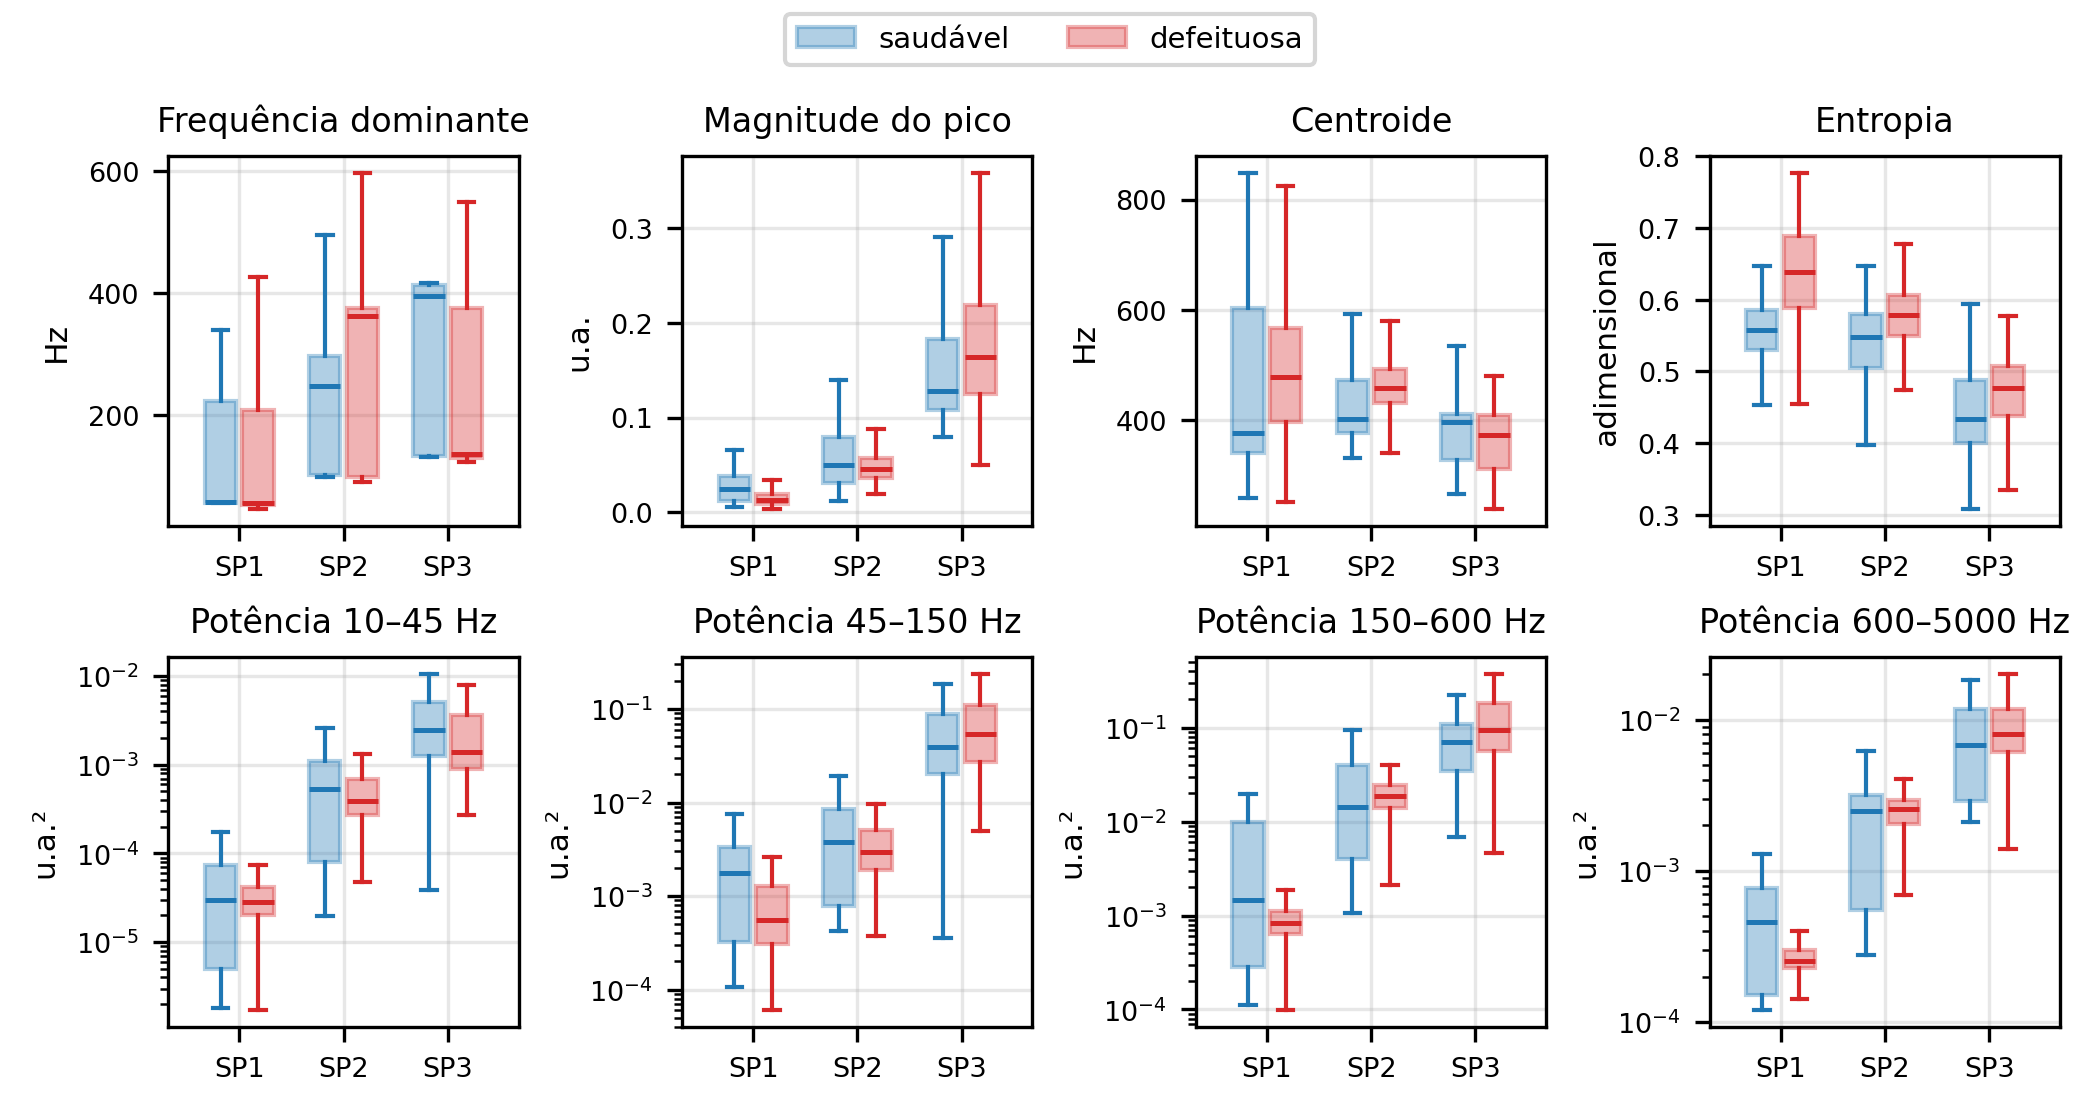
\includegraphics[width=\linewidth]{figuras/rel_box_freq.png}
  \caption{Características espectrais por janela de 2\,s, separadas por \cod{SP} (sem outliers; potências em escala log).}
  \label{fig:box_freq}
\end{figure}

\begin{table}[H]
  \centering\small
  \caption{Mediana das janelas por \cod{SP} e condição (S = saudável, D = defeituosa). Potências em $10^{-3}$\,u.a.$^2$.}
  \label{tab:freq}
  \begin{tabular}{lcccccc}
    \toprule
    & \multicolumn{2}{c}{\cod{SP1}} & \multicolumn{2}{c}{\cod{SP2}} & \multicolumn{2}{c}{\cod{SP3}} \\
    \cmidrule(lr){2-3}\cmidrule(lr){4-5}\cmidrule(lr){6-7}
    & S & D & S & D & S & D \\
    \midrule
    $f_\text{dom}$ (Hz) & 56,8 & 56 & 248 & 363 & 396 & 136 \\
    Magnitude do pico (u.a.) & 0,025 & 0,013 & 0,050 & 0,046 & 0,128 & 0,164 \\
    Potência 10--45\,Hz & 0,030 & 0,029 & 0,54 & 0,40 & 2,5 & 1,4 \\
    Potência 45--150\,Hz & 1,77 & 0,56 & 3,82 & 2,97 & 39,8 & 54,2 \\
    Potência 150--600\,Hz & 1,48 & 0,82 & 14,4 & 18,9 & 70,9 & 95,1 \\
    Potência 600--5000\,Hz & 0,46 & 0,25 & 2,51 & 2,58 & 6,79 & 8,08 \\
    Centroide (Hz) & 376 & 477 & 402 & 458 & 396 & 373 \\
    Entropia & 0,558 & 0,639 & 0,548 & 0,579 & 0,433 & 0,477 \\
    \bottomrule
  \end{tabular}
\end{table}

\textbf{Interpretação} (Figura~\ref{fig:box_freq}, Tabela~\ref{tab:freq}).
\begin{itemize}
  \item \textbf{$f_\text{dom}$ é instável.} O maior pico do espectro inteiro salta entre $f_1$ e picos mais altos da série: de 31\% a 64\% das janelas têm $f_\text{dom} > 200$\,Hz.
  \item \textbf{A magnitude do pico e as potências em banda acompanham a intensidade.} São menores na defeituosa em \cod{SP1}, próximas em \cod{SP2} e maiores em \cod{SP3}, como o RMS.
  \item \textbf{O centroide também muda de sentido} entre os \cod{SP}.
  \item \textbf{A entropia é maior na defeituosa nos três \cod{SP}.} A energia da defeituosa está menos concentrada em poucos picos.
  \item \textbf{O que o espectro revela e o gráfico temporal não mostra:} a série de picos e seu deslocamento com o \cod{SP}, a série da defeituosa em frequências mais baixas e o espalhamento da energia. Isso aparece até em \cod{SP2}, onde o RMS das duas condições é igual.
\end{itemize}

\textbf{Resolução espectral} (Figura~\ref{fig:res_alias}, em cima). No registro \cod{F0\_SV0\_SP1\_C1\_R1}, comparamos trechos de 0,2\,s e de 2\,s com o mesmo início.
Com 0,2\,s ($N = 2000$, $\Delta f = 5$\,Hz), os picos em 56,5 e 64\,Hz se fundem num só, em 55\,Hz.
Com 2\,s ($\Delta f = 0{,}5$\,Hz), eles aparecem separados.
Como $\Delta f = 1/T$ depende só da duração do trecho, separar picos próximos ou medir diferenças de poucos hertz entre condições (Seção~\ref{sec:investigacao}) exige trechos longos.
Por isso usamos janelas de 2\,s.

\textbf{Aliasing} (Figura~\ref{fig:res_alias}, embaixo). No registro \cod{F0\_SV0\_SP2\_C1\_R1}, reduzimos a taxa de 10\,kHz para \textbf{625\,Hz} (fator 16, Nyquist de 312,5\,Hz).
\begin{itemize}
  \item \textbf{Sem filtro} (\cod{x[::16]}), as componentes acima do Nyquist aparecem em $f_\text{ap} = |f - k f_s'|$: 395\,Hz vira 230\,Hz, e 494\,Hz vira 131\,Hz. A magnitude é praticamente a mesma (0,0264 contra 0,0268), e nada no espectro indica que esses picos são falsos.
  \item \textbf{Com filtro passa-baixa antes} (\cod{decimate}), os picos abaixo do Nyquist (38,5, 99 e 198\,Hz) ficam iguais, e os falsos somem (em 230\,Hz, a magnitude cai para 0,0013).
\end{itemize}
Pelo critério de Nyquist, só componentes abaixo de $f_s'/2$ são representadas corretamente.
As demais se dobram para dentro da faixa, a menos que sejam removidas antes da amostragem.

\begin{figure}[H]
  \centering
  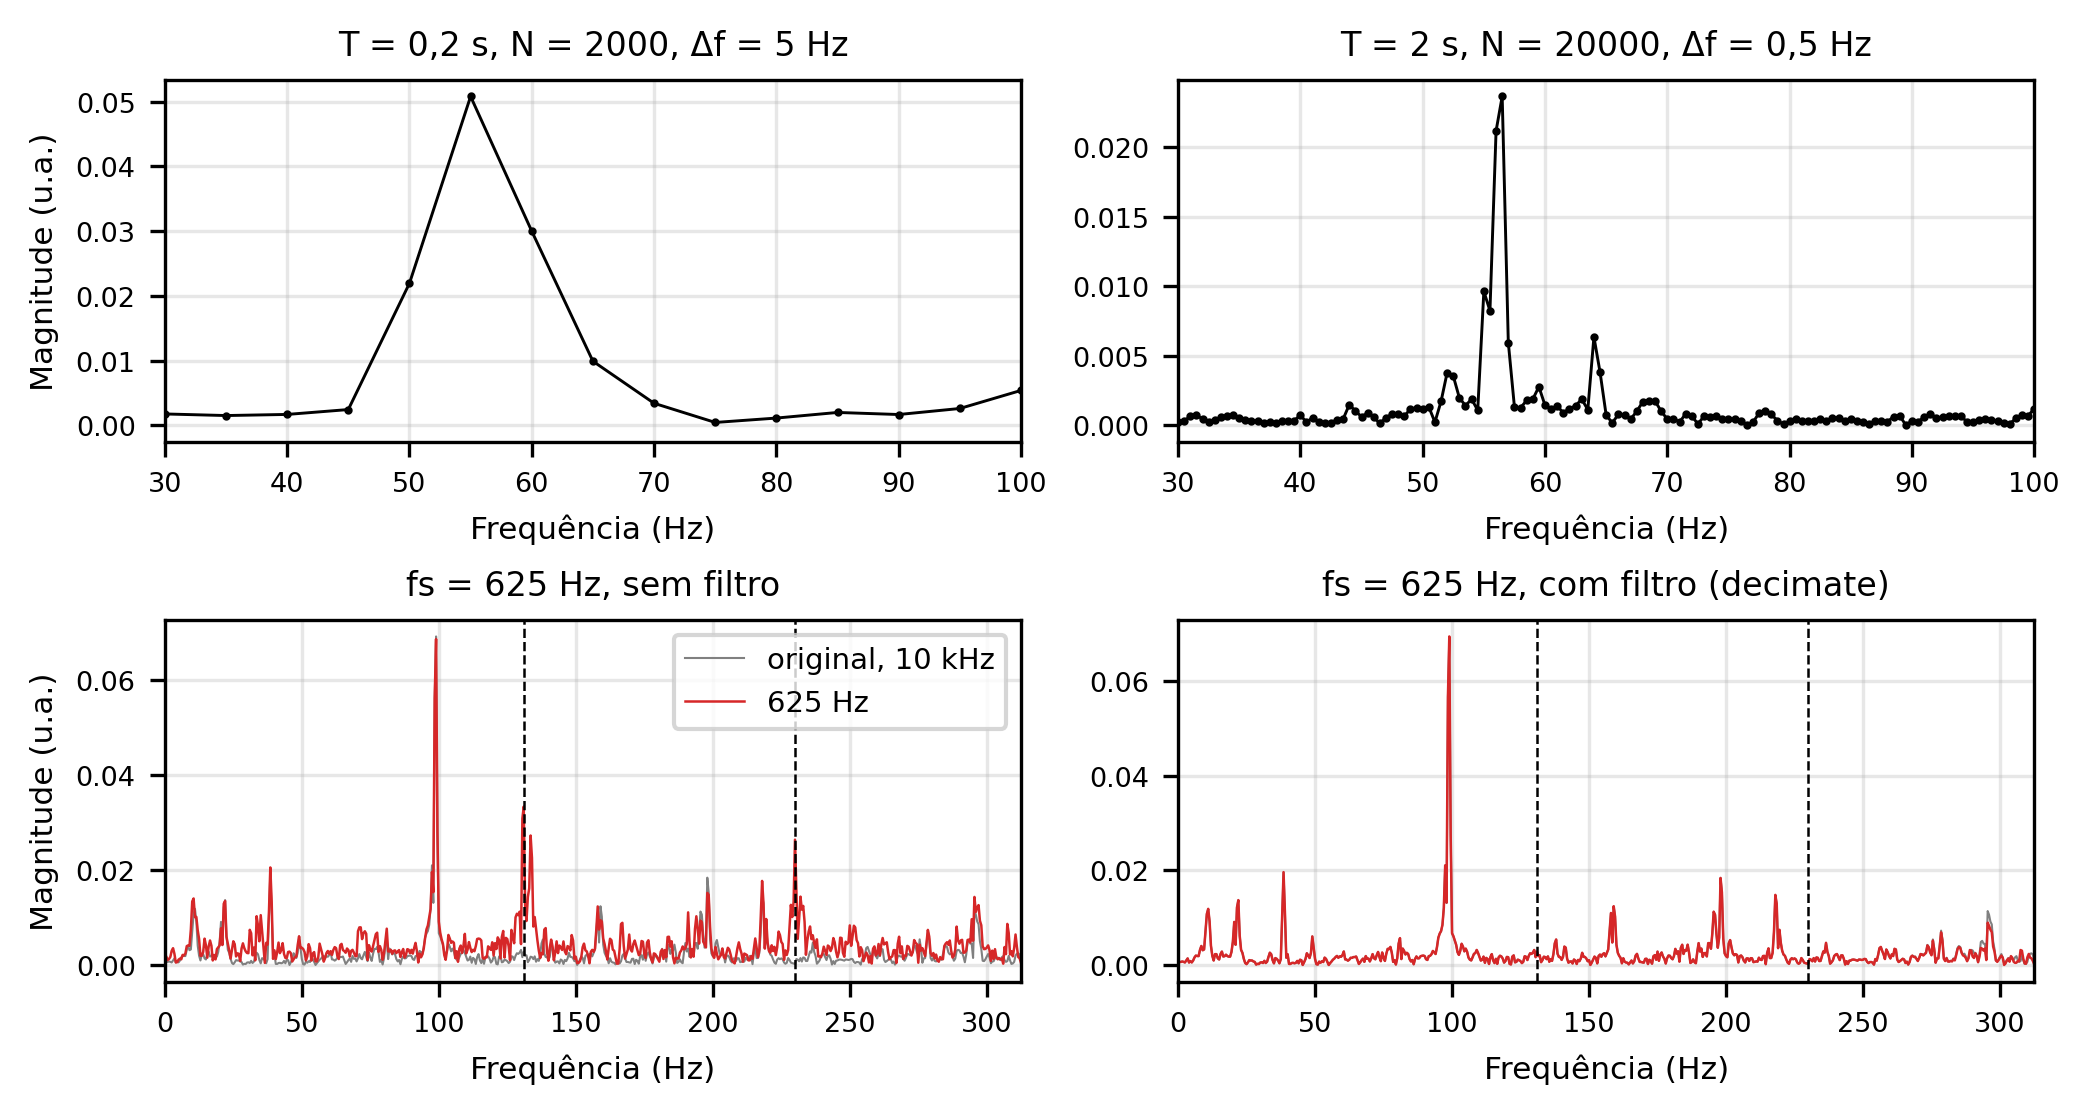
\includegraphics[width=0.92\linewidth]{figuras/rel_resolucao_aliasing.png}
  \caption{Em cima: o mesmo trecho com 0,2\,s e 2\,s. Embaixo: espectro original (cinza) e reduzido para 625\,Hz (vermelho), sem e com filtro. Tracejado: frequências aparentes previstas para 395 e 494\,Hz.}
  \label{fig:res_alias}
\end{figure}

% ------------------------------------------------------------------ 5
\section{Comparação entre domínios}
\label{sec:comparacao}

Os dois domínios usam as mesmas 2370 janelas.
Para medir a separação, calculamos a AUC (estatística $U$ de Mann--Whitney dividida por $n_D n_S$) sobre a mediana de cada registro, em cada \cod{SP} (Figura~\ref{fig:auc}).
AUC de 0,5 indica condições misturadas.
Chegamos a quatro achados.
\begin{enumerate}
  \item \textbf{O tempo mostra a intensidade, e a frequência mostra onde ela está.} Nos pares da Figura~\ref{fig:pares}, o RMS da defeituosa é menor em \cod{SP1} (0,033 contra 0,041) e muito maior em \cod{SP3} (0,48 contra 0,29). Já $f_1$ é menor na defeituosa nos três pares.
  \item \textbf{Os domínios são consistentes.} A soma das quatro bandas acompanha $3\sigma^2$, com razão mediana de 0,994 (de 0,82 a 1,18 entre os percentis 5 e 95). O fator 3 vem da normalização com Hann, $2N\sum w^2/(\sum w)^2 = 3$. A potência no tempo se distribui pelas bandas, como prevê o teorema de Parseval.
  \item \textbf{Nenhum domínio é claramente superior.} As medidas de amplitude dos dois domínios mudam de sentido entre os \cod{SP}. A entropia espectral é a única com o mesmo sentido nos três (AUC de 0,83, 0,65 e 0,59). O fator de crista e o centroide separam pouco.
  \item \textbf{A data se confunde com a condição.} A média do sinal tem a maior separação aparente (AUC de 0,02 a 0,27), mas acompanha a data. Em \cod{SP1} e \cod{SP2}, os saudáveis de setembro ficam dentro da faixa dos defeituosos.
\end{enumerate}

\begin{figure}[H]
  \centering
  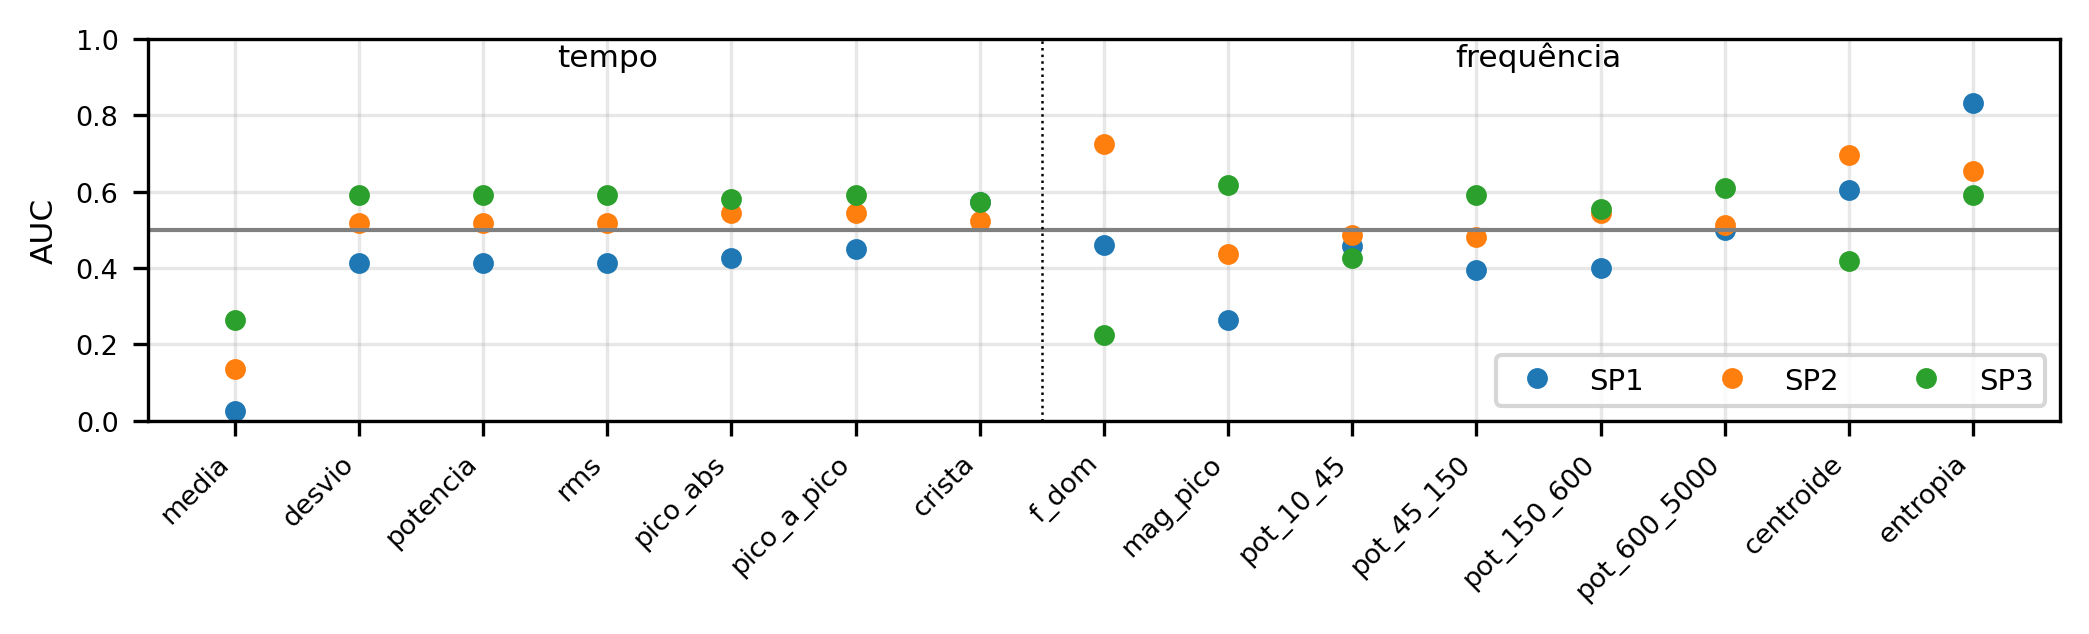
\includegraphics[width=\linewidth]{figuras/rel_auc.png}
  \caption{AUC de cada característica por \cod{SP}, sobre a mediana dos registros. Acima de 0,5, a característica tende a ser maior na defeituosa.}
  \label{fig:auc}
\end{figure}

\textbf{Redundância e conjunto para a classificação.}
\begin{itemize}
  \item No tempo, RMS, desvio e $\sqrt P$ são a mesma medida, e os picos acompanham o RMS ($\rho \ge 0{,}92$ após padronizar por \cod{SP}).
  \item Entre as espectrais, todas as correlações ficam abaixo de 0,90 em módulo.
\end{itemize}
Propomos três conjuntos:
\begin{itemize}
  \item A: RMS e fator de crista;
  \item B: as oito medidas espectrais;
  \item C: A e B juntos.
\end{itemize}
A média fica de fora, por funcionar como marcador da data.
A Seção~\ref{sec:investigacao} sugere trocar $f_\text{dom}$ por um pico de base mais estável.
A seleção será refeita só com os dados de treino.

% ------------------------------------------------------------------ 6
\section{Investigação adicional: velocidade de operação e picos espectrais}
\label{sec:investigacao}

\textbf{Pergunta.} Como varia, entre os níveis de \cod{SP}, a frequência do pico principal de 30 a 200\,Hz? A variação é a mesma nas duas condições?
A pista dos três pares da Figura~\ref{fig:pares} e a instabilidade de $f_\text{dom}$ justificam verificar isso em todos os registros.

\textbf{Método.} Em cada janela, $f_1$ é o maior pico de 30 a 200\,Hz.
Em \cod{SP1} e \cod{SP2}, ele salta entre um pico e outro com o dobro da frequência.
Por isso definimos o pico de base $f_\text{base}$: se há um pico em $f_1/2 \pm 2$\,Hz com pelo menos 30\% da magnitude de $f_1$, $f_\text{base}$ é esse pico; senão, $f_\text{base} = f_1$.
Cada registro é resumido pela mediana das janelas, e as condições são comparadas pela AUC em cada \cod{SP}.

\begin{figure}[H]
  \centering
  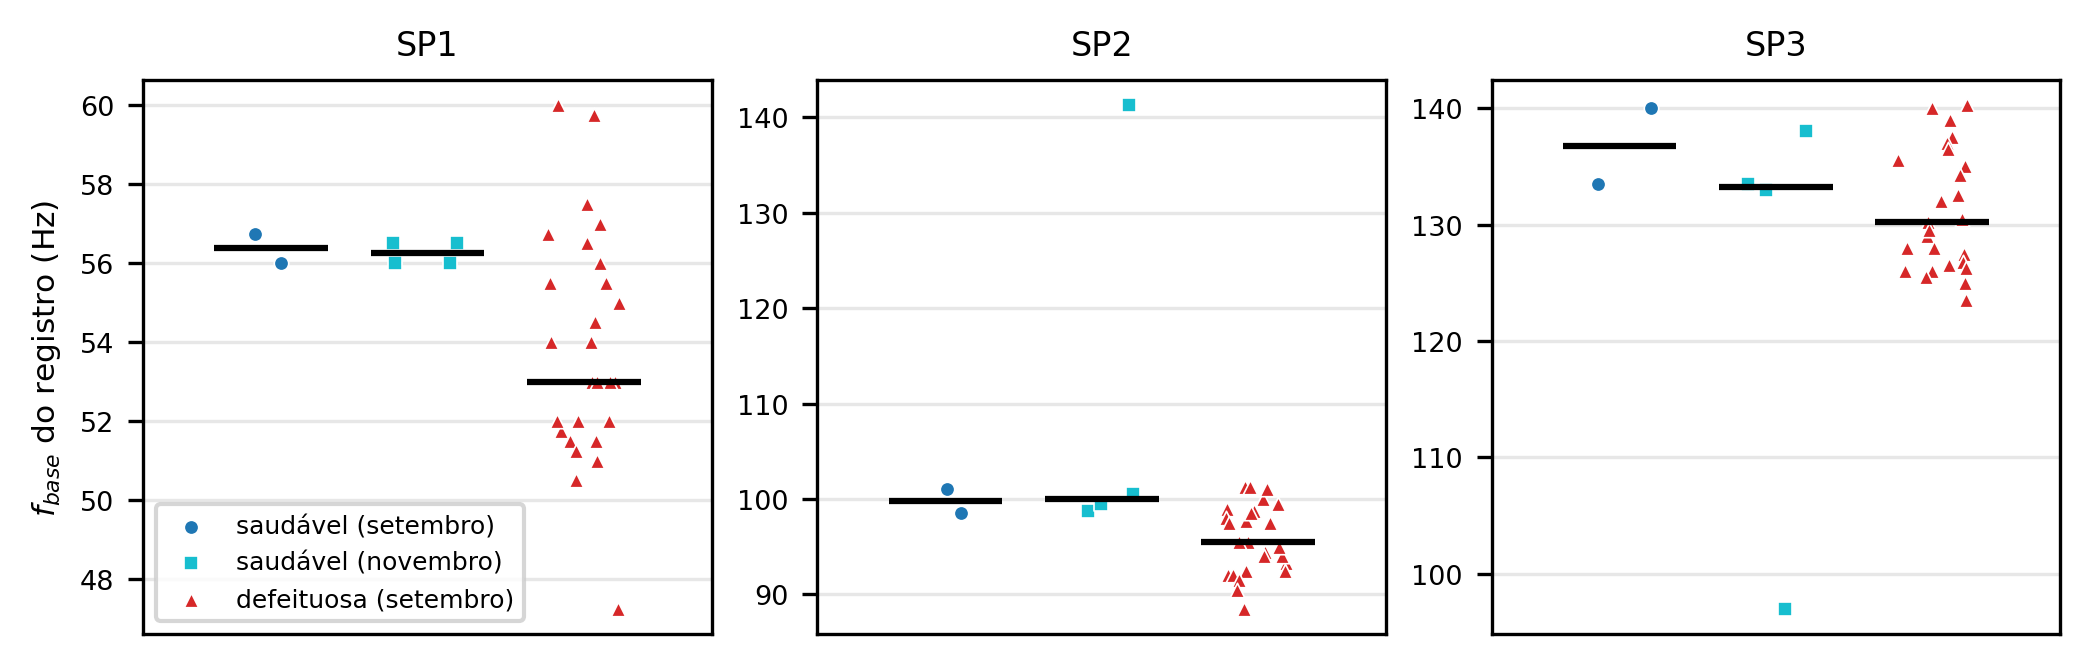
\includegraphics[width=\linewidth]{figuras/rel_picos_sp.png}
  \caption{$f_\text{base}$ de cada registro (mediana das janelas), com os saudáveis separados por mês de gravação. Traço: mediana do grupo.}
  \label{fig:picos}
\end{figure}

\begin{table}[H]
  \centering\small
  \caption{$f_\text{base}$ por \cod{SP} (mediana dos registros). A última coluna compara os defeituosos só com os saudáveis de setembro.}
  \label{tab:picos}
  \begin{tabular}{cccccc}
    \toprule
    \cod{SP} & Saudável (Hz) & Defeituosa (Hz) & Diferença & AUC & AUC (setembro) \\
    \midrule
    1 & 56,2 & 53,0 & $-5{,}8\%$ & 0,22 & 0,20 \\
    2 & 100,0 & 95,5 & $-4{,}5\%$ & 0,15 & 0,19 \\
    3 & 133,5 & 130,2 & $-2{,}4\%$ & 0,38 & 0,21 \\
    \bottomrule
  \end{tabular}
\end{table}

\textbf{Resultados} (Figura~\ref{fig:picos}, Tabela~\ref{tab:picos}).
\begin{itemize}
  \item \textbf{$f_\text{base}$ sobe com o \cod{SP}} nas duas condições, em 97 dos 99 registros. As duas exceções são saudáveis com metade das janelas em cada um de dois picos, em que a mediana cai entre eles. As razões em relação a \cod{SP1} são $\approx 1{,}8$ e $\approx 2{,}4$, e não as interpretamos sem a rotação real.
  \item \textbf{A defeituosa tem $f_\text{base}$ de 2 a 6\% menor nos três \cod{SP}} e varia mais entre registros. Em \cod{SP1}, os saudáveis ficam entre 56,0 e 56,8\,Hz, e 74\% dos defeituosos ficam abaixo disso.
  \item \textbf{A data não explica a diferença.} Os saudáveis de setembro têm o mesmo $f_\text{base}$ que os de novembro em \cod{SP1} e \cod{SP2}, e a AUC usando só eles mantém o sentido.
  \item \textbf{O resultado não depende do estimador.} Com $f_1$ sem correção, ou com limiares de 20\% e 50\%, a defeituosa continua abaixo da saudável nos três \cod{SP}.
\end{itemize}

\textbf{Conclusão.} O aumento da velocidade desloca toda a série de picos para frequências mais altas.
A hélice defeituosa tem a série ligeiramente mais baixa em todos os níveis, e é a diferença mais consistente que encontramos.
Não atribuímos causa física: a rotação de cada \cod{SP} é desconhecida, há só 6 saudáveis por nível (2 de setembro), e a classe defeituosa mistura tipos e severidades.

% ------------------------------------------------------------------ 7
\section{Conclusões}

\begin{itemize}
  \item As medidas de intensidade, no tempo ou em bandas, não separam as condições de forma consistente: o sentido muda com o \cod{SP}, e elas sofrem efeito da configuração \cod{C} e da data de gravação.
  \item O espectro revela o que o tempo não mostra. A defeituosa tem a série de picos em frequências 2 a 6\% mais baixas e a energia mais espalhada (entropia maior), com o mesmo sentido nos três níveis de velocidade.
  \item Na classificação, a divisão treino/teste será feita por registro, e o desempenho também será avaliado só com registros de setembro, por causa da confusão entre data e condição.
\end{itemize}

% ------------------------------------------------------------------ referências
\begin{thebibliography}{9}
\bibitem{dronepropb} DronePropB: Ground Testing Dataset for Commercial Drones with Defective Propellers. Mendeley Data, v1. DOI: \href{https://doi.org/10.17632/xkvfjmm8zg.1}{10.17632/xkvfjmm8zg.1}.
\bibitem{dronepropa} M.~A.~A.~Ismail, M.~E.~Elshaar, A.~Abdallah, Q.~Quan. DronePropA: Motion trajectories dataset for defective drones. \emph{Data in Brief}, v.~60, 2025. DOI: \href{https://doi.org/10.1016/j.dib.2025.111589}{10.1016/j.dib.2025.111589}.
\bibitem{plano} Plano de Ensino CIN0020 -- Sinais e Sistemas, 2026.2.
\end{thebibliography}

\end{document}
